\documentclass[%
    school=etsisi,%
    type=pfg,%
    degree=61CI,%
]{upm-report}

\setcounter{tocdepth}{1} % para ver si se incluyen subsecciones o no cambiar el depthde 1 a 2

\newcommand{\elvi}[2][inline]{\color{violet} [EAD]: #2\color{black}}

%%%%%%%%%%%%%%%%%%%%%%%%%%%%%%%%%%%%%%%%%%%%%%%%%%%%%%%%%%%%%%%%%%%%%%%%
% TÍTULO, AUTORES Y DIRECTORES
%
\title{PANOT: Plataforma Móvil para la Gestión de la Inteligencia Relacional mediante Captura Asistida de Interacciones}
\author{Ángel Rodríguez Morán}
\bibauthor{}
\director{Elvira Amador Domínguez}

%%%%%%%%%%%%%%%%%%%%%%%%%%%%%%%%%%%%%%%%%%%%%%%%%%%%%%%%%%%%%%%%%%%%%%%%
% RESUMEN Y ABSTRACT
%
\abstract{spanish}{
   mas a delante...

}
\keywords{spanish}{
    
}

\abstract{english}{
    [Write here the project summary in English]
}
\keywords{english}{
}

% Opcional
\reportquotation{
    [Cita opcional para el proyecto]
}{[Autor de la cita]}

% Opcional
\acknowledgements{
    [Escribir aquí los agradecimientos del proyecto]
}

%%%%%%%%%%%%%%%%%%%%%%%%%%%%%%%%%%%%%%%%%%%%%%%%%%%%%%%%%%%%%%%%%%%%%%%%
% GLOSARIO Y ABREVIATURAS
%
% Añadir aquí las entradas del glosario y acrónimos necesarios para el proyecto
\newglossaryentry{inferencia-analogica}{
        name=Inferencia Analógica,
        description={
            Transmisión de conocimientos de una situación a otra.
        }
}
\newglossaryentry{generalizacion-de-cero-disparos}{
        name=Generalización de Cero Disparos,
        description={
            Escenario de aprendizaje automático en el que se entrena un modelo de IA para reconocer y categorizar 
            objetos o conceptos sin haber visto ningún ejemplo de esas categorías o conceptos de antemano.
        }
}

\newglossaryentry{aes-256}{
        name=AES-256,
        description={
            Estándar de Cifrado Avanzado (Advanced Encryption Standard) que utiliza una longitud de clave de 256 bits. 
            Es uno de los algoritmos de cifrado simétrico más seguros y utilizados actualmente para proteger información 
            clasificada y datos sensibles.
        }
}

\newglossaryentry{transport-layer-security}{
        name=Transport Layer Security,
        description={
            Protocolo de seguridad que proporciona autenticación, integridad y confidencialidad de los datos en tránsito 
            entre dos puntos, generalmente entre un cliente y un servidor.
        }
}

\newglossaryentry{row-level-security}{
        name=Row Level Security,
        description={
            Mecanismo de seguridad que permite controlar el acceso a las filas de una tabla de base de datos según el usuario 
            que realiza la consulta.
        }
}

\newglossaryentry{column-level-security}{
        name=Column Level Security,
        description={
            Mecanismo de seguridad que permite controlar el acceso a las columnas de una tabla de base de datos según el usuario 
            que realiza la consulta.
        }
}

\newglossaryentry{soc-2-type-2}{
        name=SOC 2 Type 2,
        description={
            Estándar de auditoría desarrollado por el AICPA (Instituto Americano de Contadores Públicos Certificados) que 
            revisa y verifica tanto el diseño como el funcionamiento efectivo de los controles de seguridad implementados 
            por una organización para salvaguardar los datos de sus clientes durante un intervalo determinado, generalmente 
            comprendido entre 3 y 12 meses.
        }
}

\newglossaryentry{analisis-cohorte}{
        name=Análisis de Cohorte,
        description={
            Técnica de análisis de datos que divide a un grupo de individuos en subgrupos basados en características comunes 
            y observa cómo evolucionan estos individuos a lo largo del tiempo.
        }
}

\newglossaryentry{embudos}{
        name=Embudos,
        description={
            Técnica de análisis de datos que permite visualizar cómo los usuarios interactúan con diferentes partes de un producto 
            a lo largo del tiempo, ayudando a identificar patrones de retención y conversión.
        }
}

\newglossaryentry{construir-medir-aprender}{
        name=Construir-Medir-Aprender,
        description={
            Ciclo de retroalimentación fundamental de la metodología \textit{Lean Startup} diseñado para transformar ideas en productos (Construir), 
            evaluar la reacción de los clientes mediante datos (Medir) y validar o refutar hipótesis para decidir si perseverar o 
            pivotar (Aprender), con el objetivo de acelerar el aprendizaje validado y minimizar el desperdicio.
        }
}

\newglossaryentry{eliminar-desperdicio}{
        name=Eliminar Desperdicio,
        description={
            Principio de Lean Development que se basa en eliminar cualquier esfuerzo o característica que no genere valor para el usuario.
        }
}

\newglossaryentry{optimizar-todo}{
        name=Optimizar el Todo,
        description={
            Principio de Lean Development que se basa en la idea de enfocarse en mejorar el proceso completo en lugar de solo partes aisladas.
        }
}

\newglossaryentry{api-gateway}{
        name=API Gateway,
        description={
            Patrón de diseño que actúa como punto de entrada único (entry point) para un sistema distribuido, encargándose de 
            desacoplar al cliente de la implementación interna mediante la gestión centralizada del enrutamiento, la seguridad y la composición de protocolos.
        }
}

\newglossaryentry{pci-dss}{
        name=PCI DSS,
        description={
            Standard de seguridad que recoge una serie de normas obligatorias para cualquier organización que procese, acepte, 
            almacene o transite datos de tarjetas de crédito.
        }
}


\newacronym[
description={Sistema de Gestión de Relaciones con Clientes},
longplural={Customer Relationship Management}
]{crm}{CRM}{Customer Relationship Management}

\newacronym[
description={Producto Mínimo Viable},
longplural={Productos Mínimos Viables}
]{mvp}{MVP}{Producto Mínimo Viable}

\newacronym[
description={Gestión de Relaciones Personales},
longplural={Gestión de Relaciones Personales}
]{prm}{PRM}{Gestión de Relaciones Personales}

\newacronym[
description={Interfaz de Programación de Aplicaciones},
longplural={Interfaces de Programación de Aplicaciones}
]{api}{API}{Interfaz de Programación de Aplicaciones}

\newacronym[
description={Kit de Desarrollo de Software},
longplural={Kits de Desarrollo de Software}
]{sdk}{SDK}{Kit de Desarrollo de Software}

\newacronym[
description={Inteligencia Artificial},
longplural={Inteligencias Artificiales}
]{ia}{IA}{Inteligencia Artificial}

\newacronym[
description={Work In Progress},
longplural={Work In Progress}
]{wip}{WIP}{Work In Progress}

\newacronym[
description={JSON Web Token},
longplural={JSON Web Tokens}
]{jwt}{JWT}{JSON Web Token}







\begin{document}

%%%%%%%%%%%%%%%%%%%%%%%%%%%%%%%%%%%%%%%%%%%%%%%%%%%%%%%%%%%%%%%%%%%%%%%%
% CAPÍTULOS

\chapter{Introducción}
\label{ch:introduccion}

\section{Motivación}
\label{s:motivacion}

La idea de este proyecto radica de una necesidad común tanto en el ámbito personal como en el profesional: la limitación que tiene el cerebro de retener detalles o contextos específicos de las 
numerosas interacciones sociales que nos ocurren en nuestro día a día. Las soluciones actuales para satisfacer esta necesidad están muy polarizadas, o bien son soluciones muy orientadas al 
ambito profesional para personal de departamentos de ventas u otros, o bien son soluciones muy estáticas y simples como las aplicaciones de contactos en nuestros teléfonos móviles que no 
permiten capturar la evolución y el matiz de una relación interpersonal.

PANOT nace con el propósito de ocupar este hueco mediante el concepto de Inteligencia Relacional. El proyecto abarca el ciclo completo de ingeniería de software, desde el análisis de requisitos y el diseño 
de su arquitectura hasta el desarrollo y lanzamiento comercial de una aplicación móvil. Además de la solución técnica, se pretende que esta memoria en su conjunto permitiría validar y documentar un 
flujo de trabajo que transformase cualquier solución del 0 al 1 \cite{thiel2014zerotoone}, es decir, de una idea a algo tangible, y para que cualquier persona que quiera hacer lo mismo, sirva 
como guía o inspiración para hacerlo. 
\section{Objetivos del Proyecto}
\label{s:objetivos}

El objetivo general de este proyecto es diseñar, desarrollar y lanzar un \acrfull{mvp} que sirva como instrumento técnico para validar las hipótesis de valor 
asociadas al propósito de PANOT. Para alcanzar este objetivo general, se han definido los siguientes objetivos específicos:

\begin{itemize}
    \item \textbf{O1}\label{o1}. Investigar y fundamentar el paradigma de la Inteligencia Relacional, analizando las carencias de las soluciones actuales de gestión de contactos para proponer un modelo de datos basado en grafos que capture el contexto de una persona.
    \item \textbf{O2}\label{o2}. Desarrollar un motor de procesamiento semántico basado en agentes de \acrfull{ia}, que sea capaz de automatizar la extracción de entidades y relaciones a partir de lenguaje natural, reduciendo la carga cognitiva del usuario en la fase de registro.
    \item \textbf{O3}\label{o3}. Diseñar una arquitectura de software con enfoque \textit{local-first}, garantizando la soberanía del dato y la disponibilidad total de la herramienta en escenarios de movilidad o ausencia de conectividad.
    \item \textbf{O4}\label{o4}. Implementar una experiencia de usuario \textit{voice-first}, permitiendo demostrar que el uso de este tipo de interfaces de voz es la solución técnica más eficiente para minimizar la fricción en la entrada de datos por parte del usuario.
    \item \textbf{O5}\label{o5}. Instrumentar al sistema para la validación de la viabilidad técnica y económica de un sistema agentico en producción, monitorizando el rendimiento, la latencia y los costes operativos para asegurar que el modelo propuesto es sostenible y escalable.
    \item \textbf{O6}\label{o6}. Garantizar la privacidad y seguridad del usuario desde el diseño (\textit{Privacy and Efficiency by Design}), implementando mecanismos de aislamiento de datos y anonimización de métricas que protejan la información sensible gestionada por el sistema.
    \item \textbf{O7}\label{o7}. Ejecutar el ciclo completo de lanzamiento comercial en la \textit{App Store}, validando el cumplimiento de las normativas de calidad exigidas por Apple.
\end{itemize}


\section{Estructura de la memoria}
\label{s:estructura-memoria}

A modo de apoyo al lector, la presente memoria sigue una secuencia lógica organizada en los siguientes capítulos:

\begin{itemize}
    \item \textbf{Capítulo 1. Introducción} 
    \item \textbf{Capítulo 2. Estado de la Técnica}: Analizar las soluciones actuales y conceptos fundamentales sobre Inteligencia Relacional y Privacidad y Eficiencia por Diseño.
    \item \textbf{Capítulo 3. Contexto Tecnológico}: Enmarca las tecnologías y herramientas usadas durante el desarrollo del proyecto.
    \item \textbf{Capítulo 4. Desarrollo del Proyecto}: Documenta el ciclo de vida del sistema software que se pretende desarrollar (análisis - diseño - implementación - pruebas - despliegue).
    \item \textbf{Capítulo 5. Resultados y Verificación}: Expone los flujos principales del sistema, la verificación del cumplimiento de los requisitos impuestos en la fase de análisis y la discusión de los resultados.
    \item \textbf{Capítulo 6. Conclusiones}
\end{itemize}


\chapter{Estado de la Técnica y Fundamentos Tecnológicos}
\label{ch:estado-del-arte-y-fundamentos-tecnologicos}


\section{Gestión de la Inteligencia Relacional}

Los sistemas \acrshort{crm} convencionales, si bien útiles en entornos corporativos para la gestión masiva de clientes, presentan 
limitaciones significativas cuando se trata de capturar la complejidad inherente a las relaciones humanas. Estos sistemas 
operan principalmente con información descontextualizada, almacenando datos de contacto de manera estática y registrando 
interacciones sin considerar su evolución temporal ni el contexto en el que ocurren.

La Inteligencia Relacional presenta un nuevo paradigma evolutivo en la gestión de información personal y profesional, introduciendo el
concepto de dinamismo contextual, donde cada relación evoluciona continuamente reflejando cambios en intereses, preferencias y circunstancias vitales. 
Este enfoque reconoce que las relaciones que tenemos no son entidades fijas, sino procesos complejos que cambian según un contexto temporal y situacional.


\subsection{Inteligencia Relacional en el Contexto de la Inteligencia Artificial}

Para comprender el alcance de la Inteligencia Relacional, es necesario enmarcar el concepto dentro del ecosistema más amplio
de la Inteligencia Artificial y analizar cómo se diferencia con los paradigmas tradicionales.

La diferencia fundamental entre la Inteligencia Relacional y los paradigmas tradicionales de IA radica en que, mientras estos últimos 
operan principalmente mediante la aproximación estadística de distribuciones de datos y patrones —optimizando funciones de pérdida sobre grandes volúmenes 
de datos descontextualizados—, la Inteligencia Relacional se fundamenta en la construcción y manipulación de representaciones 
estructurales de relaciones que permiten la generalización cruzada y la \gls{inferencia-analogica}. 
La Inteligencia Relacional captura la estructura relacional subyacente que puede transferirse entre dominios aparentemente no relacionados, 
tal como ocurre en el razonamiento humano, creando un contexto de conocimiento más amplio y generalizable o especfíco para un dominio en concreto.

La investigación en Inteligencia Relacional demuestra capacidades que van más allá del aprendizaje estadístico tradicional. 
En 2022, se publicó un estudio de la Universidad de Edimburgo\cite{doumas2022theory} en el que se muestra cómo un modelo computacional puede aprender representaciones relacionales 
estructuradas y realizar \gls{generalizacion-de-cero-disparos} entre dominios completamente diferentes, como la transferencia de 
conocimiento entre videojuegos. Esta capacidad de generalización permite que el sistema aprenda a reconocer y comprender relaciones 
entre entidades en contextos completamente diferentes.

Traspasando la analogía de los videojuegos al contexto de PANOT, la Inteligencia Relacional como se menciona en \cite{doumas2022theory} permite que el sistema
aprenda a reconocer y comprender patrones relacionales estructurados entre personas, eventos y contextos, más allá de las asociaciones estadísticas superficiales. 
En lugar de simplemente almacenar datos estáticos de contactos, el sistema de PANOT puede construir representaciones relacionales dinámicas que capturan la estructura subyacente 
de las relaciones humanas —como la evolución temporal de intereses comunes, la frecuencia contextual de interacciones, o los cambios en preferencias y circunstancias vitales—. 

Para ilustrar este proceso, consideremos un ejemplo práctico del flujo de procesamiento relacional en PANOT:

\textit{Input:} El usuario captura una interacción mediante nota de voz: ``Acabo de almorzar con María. Está muy emocionada 
porque ha conseguido un nuevo trabajo como diseñadora en una startup tecnológica. Le interesa especialmente el trabajo remoto 
y mencionó que está buscando un piso más cerca de su nueva oficina. Hablamos de proyectos de diseño colaborativo y se mostró 
muy receptiva a la idea de futuros proyectos juntos.''

\textit{Procesamiento:} PANOT procesa esta entrada multimodal extrayendo múltiples capas de información relacional 
estructurada:

{\small
\begin{itemize}
    \setlength{\itemsep}{0pt}
    \setlength{\parsep}{0pt}
    \setlength{\topsep}{0pt}
    \setlength{\partopsep}{0pt}
    \item \textit{Evento}: almuerzo social de contexto informal
    \item \textit{Cambio de estado}: transición profesional — nuevo trabajo como diseñadora
    \item \textit{Cambio de preferencias}: prioridad hacia trabajo remoto
    \item \textit{Necesidad emergente}: búsqueda de vivienda
    \item \textit{Relaciones}: interés común en proyectos de diseño colaborativo, receptividad a futura colaboración
    \item \textit{Contexto temporal}: estado emocional positivo, momento de transición vital
\end{itemize}
} 

El sistema construye una representación relacional estructurada que conecta estas entidades (usuario-contacto)
mediante relaciones semánticas representadas en formato \texttt{JSON}:

\begin{lstlisting}[
    basicstyle=\ttfamily\scriptsize,
    breaklines=true,
    breakatwhitespace=false,
    keepspaces=true,
    showspaces=false,
    showstringspaces=false,
    tabsize=2
]
{
  "personal": {
    "necesidad_actual": "búsqueda de vivienda",
    "preferencia_ubicación": "cerca de la nueva oficina",
    "estado_emocional": "emocionada"
  },
  "profesional": {
    "rol": "diseñadora",
    "empresa": "startup tecnológica",
    "intereses": ["trabajo remoto"],
    "estado": "transición laboral reciente"
  },
  "relación": {
    "última_interacción": "almuerzo informal",
    "intereses_comunes": ["diseño colaborativo", "proyectos futuros"],
    "dinámica": "receptiva a colaboración"
  }
}
\end{lstlisting}

\textit{Output:} PANOT actualiza dinámicamente el contexto de María, integrando la nueva información estructurada directamente en su perfil relacional:

{\small
\begin{itemize}
    \setlength{\itemsep}{0pt}
    \setlength{\parsep}{0pt}
    \setlength{\topsep}{0pt}
    \setlength{\partopsep}{0pt}
    \item \textit{Contexto Personal}: Se actualiza el estado vital reflejando la necesidad activa de ``búsqueda de vivienda'' y su preferencia de ubicación, además de capturar el estado emocional positivo asociado al cambio.
    \item \textit{Contexto Profesional}: Se modifica la información laboral para incluir el nuevo rol de ``diseñadora en startup tecnológica'' y se añade el ``trabajo remoto'' como un interés profesional clave en esta etapa.
    \item \textit{Contexto de la Relación}: Se enriquece la dinámica de la relación registrando los ``proyectos de diseño colaborativo'' como un nuevo eje de interés común y actualizando el estado de la relación hacia una posible colaboración futura.
\end{itemize}
}

Así, el contacto de María dentro de la base de datos de PANOT quedaría como un conjunto de nodos interconectados que representan 
eventos, gustos, situaciones, necesidades, etc. abstrayéndo el complejo contexto de la relación en una representación más simplificada.

\begin{figure}
    \centering
        \includegraphics[width=1\textwidth]{figures/grafo-contexto-maria.png}
    \caption{\label{fig:fig-gf-maria} Representación orientativa en MemGraph Lab del contexto del contacto «María» en formato grafo relacional }
\end{figure}

\subsection{Arquitecturas Similares: Grafos Contextuales en Sistemas de Agentes}

La representación relacional estructurada que utiliza PANOT encuentra un paralelismo arquitectónico significativo con sistemas de agentes 
de inteligencia artificial que emplean grafos contextuales como mecanismo de memoria persistente. Estos sistemas, inspirados en arquitecturas 
como GraphRAG (Graph Retrieval-Augmented Generation), implementan grafos de conocimiento que permiten a los agentes acceder de manera 
eficiente a información estructurada y realizar razonamientos complejos mediante la navegación de relaciones semánticas.

En arquitecturas de agentes modernas, el grafo contextual actúa como una memoria estructurada que almacena información sobre interacciones 
pasadas, estados del entorno y relaciones entre diferentes entidades. Esta estructura permite a los agentes:

\begin{itemize}
    \setlength{\itemsep}{0pt}
    \setlength{\parsep}{0pt}
    \setlength{\topsep}{0pt}
    \setlength{\partopsep}{0pt}
    \item \textit{Almacenar información de forma estructurada}: Capturar y organizar datos sobre estados, eventos y relaciones de manera 
    que preserve la estructura relacional subyacente, en lugar de almacenar información de forma descontextualizada.
    \item \textit{Acceder rápidamente a información relevante}: Navegar eficientemente por el grafo para recuperar datos pertinentes según 
    la situación actual, mejorando significativamente la eficiencia en la recuperación de información comparado con búsquedas en bases de datos 
    relacionales tradicionales.
    \item \textit{Facilitar el razonamiento complejo}: Utilizar la estructura del grafo para inferir nuevas relaciones y tomar decisiones 
    informadas mediante razonamiento multihop —la capacidad de realizar inferencias a través de múltiples pasos siguiendo las conexiones 
    del grafo—.
    \item \textit{Adaptabilidad y aprendizaje continuo}: Actualizar y expandir el conocimiento de manera dinámica, incorporando nuevas 
    interacciones y relaciones sin requerir reestructuración completa de la base de datos.
\end{itemize}

La eficiencia superior de las estructuras de grafo para la memoria de los agentes radica en la diferencia fundamental entre el modelo de 
acceso a datos relacionales y el modelo de navegación por grafos. En las bases de datos relacionales, recuperar información sobre 
relaciones entre entidades requiere realizar múltiples operaciones que pueden cruzar tablas diferentes, lo cual implica escanear 
índices y realizar comparaciones entre grandes volúmenes de datos. La complejidad de estas operaciones crece exponencialmente con el número 
de relaciones involucradas, resultando en tiempos de consulta que pueden ser $\mathcal{O}(n \log n)$ o peor cuando se requieren múltiples uniones de tablas 
anidadas. 

Por el contrario, en una estructura de grafo, acceder a los vecinos directos de un nodo —es decir, recuperar todas las relaciones 
de una entidad— es una operación de complejidad $\mathcal{O}(1)$ en promedio, ya que las conexiones están almacenadas directamente como parte de la 
estructura del nodo mediante listas de adyacencia o estructuras similares. Esta diferencia es crítica para sistemas de agentes que requieren 
acceso frecuente y rápido a información relacional.

Como ejemplo, si queremos que nuestro sistema haga una consulta relacional para recuperar ``todos los eventos relacionados con 
María y sus intereses comunes'' podría requerir de múltiples uniones de las tablas de contactos, eventos, intereses y relaciones en el caso
en el que se trate de un sistema de relacional. Por el contrario, en un grafo contextual, esta misma información se obtiene mediante una simple navegación 
a través de las aristas conectadas al nodo de María, accediendo directamente a los nodos adyacentes sin necesidad de realizar búsquedas complejas.

En el contexto de PANOT, el grafo relacional que representa cada contacto y sus interacciones funciona análogamente al grafo contextual de 
un sistema agéntico: ambos proporcionan una estructura que permite acceso eficiente a información relevante, razonamiento sobre relaciones 
complejas y actualización dinámica del conocimiento. Esta arquitectura permite que PANOT no solo almacene información sobre contactos, sino 
que también pueda realizar inferencias relacionales, generalizar patrones entre relaciones y adaptarse continuamente a la evolución de las 
interacciones humanas, aunque veremos más adelante que el enfoque de PANOT es algo diferente.


%%%%%%%%%%%%%%%%%%%%%%%%%%%%%%%%%%%
% PARADIGMAS DE DISEÑO DE PRODUCTO EN LA ERA DE LA IA

\section{Cambio de Paradigma en el Diseño de Producto}

Un paradigma de diseño de producto constituye un conjunto de principios fundamentales, patrones de interacción y enfoques 
conceptuales que guían la creación de experiencias de usuario en productos y servicios digitales o analógicos. Representa más que una 
simple metodología de diseño; es una filosofía que establece cómo los usuarios perciben, interactúan y se relacionan 
con una aplicación. Fijese que este apartado no está orientado en principios de diseño de la arquitectura del software, sino en 
principios de diseño de producto que van más allá del desarrollo de la aplicación y están orientados en la experiencia del usuario.

En el contexto de las aplicaciones móviles, la relevancia de los paradigmas de diseño de producto adquiere una dimensión crítica 
debido a las características inherentes de estos dispositivos: limitaciones de espacio en pantalla, interacciones 
predominantemente táctiles y expectativas de inmediatez y estímulo por parte de los usuarios. 
Un paradigma de diseño adecuado no solo determina la usabilidad de una aplicación, sino que establece la base sobre la 
cual se construyen las expectativas del usuario, su curva de aprendizaje y, fundamentalmente, su conexión emocional con el producto.

La irrupción de la Inteligencia Artificial como tecnología dominante ha transformado radicalmente el panorama del diseño de productos digitales. 
La democratización de las capacidades de IA ha generado un desplazamiento del valor diferencial de los productos: ya no es suficiente ofrecer una funcionalidad 
única o una interfaz atractiva, pues estas características pueden replicarse rápidamente. En este nuevo contexto, la diferenciación competitiva 
se desplaza hacia dimensiones más profundas y fundamentales de la experiencia humana.

\subsection{Valores Diferenciadores en la Era de la IA}
 
En busca de la diferenciación y lealtad a largo plazo de estos productos, se deben incorporar valores fundamentales más allá de 
la funcionalidad técnica. Para construir un producto que se diferencie, es esencial y crítico en la era en la vivimos
generar valor desde flancos más profundos y fundamentales de la experiencia humana. Como punto de partida, el producto ha de centrarse en 
en los siguientes dos principios:

{\small
\begin{itemize}
    \setlength{\itemsep}{0pt}
    \setlength{\parsep}{0pt}
    \setlength{\topsep}{0pt}
    \setlength{\partopsep}{0pt}
    \item \textit{Conexión y resonancia emocional}: El producto debe generar una conexión emocional genuina con los usuarios, 
    comprendiendo su contexto y acompañando la evolución de sus necesidades, para establecer vínculos sostenibles que trasciendan 
    la interacción funcional.
    
    \item \textit{Personalización adaptativa y comprensión contextual}: El sistema debe de tener la capacidad de aprender 
    activamente de las interacciones con el usuario, infiriendo patrones, intereses y necesidades implícitas sin requerir configuraciones 
    explícitas, y adaptando la experiencia de manera proactiva y sin fricción, asegurando una experiencia personalizada continua.
\end{itemize}
}

Los usuarios no solo buscan que una aplicación funcione bien; buscan que se \textit{adapte} a ellos, 
que \textit{comprenda} su contexto, que \textit{evolucione} con sus necesidades y que establezca una conexión 
que trascienda la mera transacción funcional.

\input{chapter2-fundamentos/3-tecnologias-ios}
%%%%%%%%%%%%%%%%%%%%%%%%%%%%%%%%%%%
% ANÁLISIS COMPARATIVO

\section{Análisis Comparativo}

[Escribir aqui el analisis comparativo]


\chapter{Desarrollo del Proyecto}
\label{ch:desarrollo-del-proyecto}

\section{Filosofía y Metodología de Desarrollo}

El desarrollo de PANOT se ha planteado desde una perspectiva que prioriza la validación empírica y la eficiencia en 
la entrega de valor, alejándose de los enfoques tradicionales de planificación predictiva en cascada. Dado el carácter 
innovador de la propuesta —la gestión de la inteligencia relacional mediante \acrshort{ia} —, el proyecto se enfrenta a un alto 
grado de incertidumbre, no tanto en la viabilidad técnica, sino en la validación del producto por parte del usuario final.

Para mitigar este riesgo, se ha adoptado una filosofía fundamentada en los principios de \textit{Lean Startup} \cite{ries2011lean}
y \textit{Lean Thinking} \cite{2012leanthinking}. Bajo este prisma, el desarrollo de software no se entiende como la ejecución de una especificación 
cerrada, sino como un proceso de descubrimiento orientado a minimizar el desperdicio (Muda) —entendido como cualquier 
esfuerzo o característica que no genere valor para el usuario.

En consecuencia, la metodología de trabajo implementada en este Trabajo Fin de Grado no tiene como objetivo la 
finalización de un producto comercial definitivo, sino la construcción y despliegue de un \acrlong{mvp}. Este \acrshort{mvp} 
constituye el punto de partida necesario para ejecutar la primera fase del ciclo \gls{construir-medir-aprender}, 
permitiendo someter a prueba las hipótesis conceptuales detalladas en el capítulo anterior y generar un aprendizaje que 
guíe la evolución futura de la plataforma. 


\subsection{Enfoque Lean} \label{sec:enfoque-lean}

Para el desarrollo del sistema, como ya hemos comentado, se ha descartado la adopción de modelos tradicionales en cascada e incluso de 
marcos ágiles rígidos como Scrum, en favor de una filosofía fundamentada en los principios de \textit{Lean Software Development}. Respondiendo así 
a la necesidad inherente de gestionar la alta incertidumbre que los productos de características similares a PANOT suponen.

Esta decisión cobra especial relevancia al considerar la naturaleza unipersonal del equipo de desarrollo. 
Mientras que metodologías como Scrum imponen una sobrecarga de gestión mediante reuniones y artefactos 
diseñados para la coordinación grupal, el enfoque Lean permite aplicar el principio de \gls{optimizar-todo}, eliminando 
la burocracia innecesaria. Esto maximiza el ancho de banda cognitivo disponible para tareas de ingeniería y diseño, permitiendo 
mantener un flujo de entrega continuo sin las interrupciones artificiales de los \textit{sprints} temporales.

Bajo esta premisa, el trabajo presentado en esta memoria no debe entenderse como un producto final inmutable, sino como la materialización de 
la fase \textit{Construir} del ciclo \gls{construir-medir-aprender}. El \acrshort{mvp} de PANOT actuará como el artefacto necesario para validar 
la hipótesis de \textit{Inteligencia Relacional} elimanando todo el desarrollo superfluo que no contribuya a esta validación, cumpliendo así con 
el principio Lean de \gls{eliminar-desperdicio}.

Así mismo, el éxito del proyecto no se cuantifica mediante el número de funcionalidades entregadas o el cumplimiento estricto de un cronograma 
predictivo, sino a través de la capacidad del sistema para generar \textit{Aprendizaje Validado}. El objetivo técnico es instrumentar la aplicación 
(capa de observabilidad) para que, en iteraciones futuras, sea posible medir con datos reales el compromiso del usuario y la utilidad de la propuesta.

\subsection{Metodología y Flujo de Desarrollo}

Para organizar de manera robusta y estable la carga de trabajo del proyecto, se ha optado por la adopción de la metodología de ramificación \textit{GitFlow}.
Este modelo se fundamenta en la segregación de responsabilidades, estableciendo dos ramas longevas principales: \texttt{main}, que contiene exclusivamente 
código estable de producción, y \texttt{development}, que actúa como entorno de integración.

El desarrollo de nuevas características se realiza de manera aislada en ramas efímeras (\texttt{feature/*}), que solo se fusionan con la rama de integración 
tras ser completadas y validadas —Ver \ref{fig:gitflow-diagram}—. Esta estrategia garantiza la estabilidad del sistema al evitar que el código en desarrollo comprometa la funcionalidad base.

\begin{figure}
    \centering
        \includegraphics[width=1\textwidth]{figures/gitflow-diagram.png}
    \caption{Diagrama orientativo de la estrategia de ramificación. 
    (1) \textbf{Aislamiento}: Creación de una rama efímera (\textit{feature}) a partir de desarrollo para trabajar en un \textit{Issue} específico. 
    (2) \textbf{Implementación}: Desarrollo de la funcionalidad mediante \textit{commits} atómicos. 
    (3) \textbf{Integración}: Fusión de la rama mediante un \textit{Pull Request} validado, cerrando el ciclo de desarrollo. 
    (4) \textbf{Release}: Promoción del código estable desde desarrollo a la rama principal (\textit{main}) para su despliegue en producción.}
    \label{fig:gitflow-diagram}
\end{figure}

Para la orquestación de las tareas, se ha utilizado GitHub Projects, implementando un tablero Kanban automatizado que permite visualizar el flujo de valor y 
limitar el trabajo en curso. La trazabilidad entre la planificación y la ejecución se articula mediante dos artefactos clave:

\begin{itemize}
    \item \textbf{Issues:} Representan las unidades de trabajo o requisitos del sistema. Cada \textit{Issue} posee un identificador único \(\#Nº\) y, 
    para organizar la granularidad del proyecto, se ha establecido una jerarquía de dos niveles:
    \begin{itemize}
        \item \textbf{[Epic] Issues:} Representan las grandes funcionalidades o módulos del sistema (Features).
        \item \textbf{FR (Functional Requirements):} Actúan como sub-tareas atómicas vinculadas a un Epic, definiendo requisitos concretos implementables en una sola iteración.
    \end{itemize}

    \item \textbf{Pull Requests (PRs):} Constituyen el mecanismo de control de calidad y fusión de código. Una vez finalizado el desarrollo en una rama 
    \texttt{feature/*}, se abre un PR hacia \texttt{development}. En el contexto de este proyecto, el PR cumple una doble función: actúa como una etapa 
    de revisión de código obligatoria —permitiendo verificar diferencias (\textit{diffs}) y detectar errores antes de la integración— y 
    sirve como disparador automático para cerrar los \textit{Issues} asociados, garantizando así la trazabilidad completa entre el 
    requisito definido y el código implementado.
\end{itemize}


Finalmente, estas tareas transitan por el tablero Kanban siguiendo un flujo de estados que refleja el ciclo de vida del desarrollo:

\begin{itemize}
    \item \textbf{Backlog}: Contiene el conjunto de \textit{Issues} pendientes de implementación. Dado que el alcance del proyecto 
    se ha limitado estrictamente al \acrshort{mvp}, todas las tareas presentes en esta columna se consideran críticas y obligatorias 
    para el funcionamiento del sistema, habiéndose descartado previamente cualquier funcionalidad accesoria.
    
    \item \textbf{In Progress}: Indica la tarea que se está codificando activamente en ese momento. Siguiendo la filosofía Lean de \gls{eliminar-desperdicio} 
    por cambio de contexto, se mantiene un límite de trabajo en curso (\gls{wip}) estricto de una única tarea simultánea.
    
    \item \textbf{In Review}: Estado en el que la funcionalidad ha sido completada y existe un \textit{Pull Request} abierto. Actúa como 
    fase de control de calidad y auto-revisión de las diferencias de código (\textit{diff}) antes de su integración.
    
    \item \textbf{Done}: Agrupa las tareas finalizadas cuyo código ha sido validado y fusionado (\textit{merged}) exitosamente en la rama 
    \texttt{develop}, cerrando así el \textit{Issue} asociado y marcando la entrega de valor.
\end{itemize}

\begin{figure}
    \centering
        \includegraphics[width=0.95\textwidth]{figures/tablero-kanban.png}
    \caption{Visualización de las columnas del tablero Kanban implementado en GitHub Projects en un punto del desarrollo. Se destaca el límite de \gls{wip}
    configurado a 1 en la columna \textit{In Progress} (indicador 1/1), forzando un flujo continuo y eliminando el 
    desperdicio asociado al cambio de contexto.}
    \label{fig:tablero-kanban}
\end{figure}


\section{Definición del PMV y Especificación de Requisitos}

Siguiendo el marco teórico expuesto por \textit{Eric Ries} \cite{ries2011lean} el desarrollo de PANOT se fundamenta en la identificación y validación de \textit{Asunciones de Salto Fe}.
Estas son las premisas de mayor incertidumbre y riesgo que, de resultar falsas, invalidarían la totalidad del proyecto.

Las dos asunciones fundamentales en este marco son:

{\small
\begin{itemize}
\setlength{\itemsep}{0pt}
    \setlength{\parsep}{0pt}
    \setlength{\topsep}{0pt}
    \setlength{\partopsep}{0pt}
    \item \textbf{Hipótesis de Valor:} Determina si un producto o servicio proporciona valor real a los usuarios una vez que lo utilizan. 
    Se valida analizando la retención y el uso voluntario y respondería a la pregunta: \textit{¿El usuario percibe suficiente utilidad en el 
    sistema como para incorporarlo a su vida diaria?}

    \item \textbf{Hipótesis de Crecimiento:} Determina cómo los nuevos usuarios descubrirán el producto o servicio. Se valida analizando 
    los motores de crecimiento (viral, pegajoso o remunerado). Responde a la pregunta: \textit{¿Existe un mecanismo sostenible para adquirir 
    nuevos usuarios y escalar el producto?}
\end{itemize}
}

A modo aclarativo, el esfuerzo de ingeniería de este Proyecto Fin de Grado se ha focalizado en la validación de la \textit{Hipótesis de Valor}, dejando
la validación de la \textit{Hipótesis de Crecimiento} para estados futuros del ciclo de vida de la aplicación.

\subsection{Hipótesis de Valor}

Teniendo en cuenta lo anterior, el artefacto para validar la \textit{Hipótesis de Valor} es un \gls{mvp} que representa la versión mínima funcional de PANOT. 
La hipótesis concreta es que los usuarios adoptarán el sistema porque resuelve la carga cognitiva y el esfuerzo manual que supone mantener relaciones 
personales. Esta hipótesis general se desglosa en tres premisas clave:

{\small
\begin{enumerate}
    \setlength{\itemsep}{0pt}
    \setlength{\parsep}{0pt}
    \setlength{\topsep}{0pt}
    \setlength{\partopsep}{0pt}
    \item \textbf{Valor de la Inmediatez:} Se asume que los usuarios serán constantes en el registro de información 
    solo si el esfuerzo requerido y la fricción son cercanos a cero. La captura por voz ofrece un valor superior a la entrada de texto tradicional al permitir 
    registrar interacciones en movimiento y sin necesidad de una atención visual exhaustiva.
    
    \item \textbf{Valor de la Mantenibilidad Pasiva:} Se asume que los usuarios perciben valor en un sistema que mantiene actualizada la información 
    de sus contactos (cambios de trabajo, mudanzas, gustos) de forma autónoma, liberándoles de la tarea administrativa de editar fichas 
    de contacto manualmente.
    
    \item \textbf{Valor de la Memoria Aumentada:} Se asume que los usuarios obtienen utilidad real al disponer de resúmenes contextuales 
    precisos antes de una interacción, mejorando así la calidad de sus relaciones sociales gracias a una "memoria externa" que procesa el contexto del contacto por ellos.
\end{enumerate}
}

Se han establecido una serie de requisitos obligatorios que instrumentarán al sistema 
con las capacidades para validar las premisas planteadas. Estos requisitos de funcionalidad 
se han agrupado en las siguientes características principales (Features): \\

\begin{table}[H]
\centering
\small
\begin{tabular}{|l|l|l|}
\hline
\rowcolor[HTML]{EFEFEF} 
\textit{ID}          & \textit{Nombre}          & \textit{Requisitos Funcionales Asociados (IDs)}                                                                                                                                     \\ \hline
\textbf{F1}          & Gestión de Usuario       & \hyperref[req:FR-01]{FR-01}, \hyperref[req:FR-02]{FR-02}, \hyperref[req:FR-03]{FR-03}                                                                                               \\ \hline
\textbf{F2}          & Gestión de Contactos     & \hyperref[req:FR-04]{FR-04}, \hyperref[req:FR-05]{FR-05}, \hyperref[req:FR-06]{FR-06}, \hyperref[req:FR-07]{FR-07}, \hyperref[req:FR-08]{FR-08}, \hyperref[req:FR-09]{FR-09}        \\ \hline
\textbf{F3}          & Gestión de Interacciones & \hyperref[req:FR-10]{FR-10}, \hyperref[req:FR-11]{FR-11}, \hyperref[req:FR-12]{FR-12}, \hyperref[req:FR-13]{FR-13}                                                                  \\ \hline
\textbf{F4}          & Inteligencia Relacional  & \hyperref[req:FR-14]{FR-14}, \hyperref[req:FR-15]{FR-15}                                                                                                                            \\ \hline
\textbf{F5}          & Soporte y Feedback       & \hyperref[req:FR-16]{FR-16}, \hyperref[req:FR-17]{FR-17}                                                                                                                            \\ \hline
\end{tabular}
\caption{Features del Sistema y los IDs de los Requisitos Funcionales Asociados}
\label{tab:system-features}
\end{table}

\subsection{Requisitos Funcionales}

\begin{table}[H]
\scriptsize
\begin{tabularx}{\textwidth}{|l|X|}
\hline
\rowcolor[HTML]{EFEFEF} 
\textit{ID}                            & \textit{Descripción} \\ \hline
\textbf{FR-01} \label{req:FR-01}       & El sistema debe permitir el registro e inicio de sesión de usuarios de forma segura. \\ \hline
\textbf{FR-02} \label{req:FR-02}       & El sistema debe permitir cerrar sesión al usuario de forma segura. \\ \hline
\textbf{FR-03} \label{req:FR-03}       & El sistema debe permitir al usuario la eliminación completa de su cuenta y toda la información asociada a ella, lo que debe desencadenar el borrado de sus datos tanto en el dispositivo local como en el servidor remoto. \\ \hline
\end{tabularx}
\caption{Requisitos Funcionales de la \hyperref[tab:system-features]{\textit{Feature 1 - Gestión de Usuario}}}
\label{tab:functional-requirements-f1}
\end{table}

\begin{table}[H]
\scriptsize
\begin{tabularx}{\textwidth}{|l|X|}
\hline
\rowcolor[HTML]{EFEFEF} 
\textit{ID}                            & \textit{Descripción} \\ \hline
\textbf{FR-04} \label{req:FR-04}       & El sistema debe permitir dar de alta un contacto manualmente introduciendo, al menos, un nombre identificativo y adicionalmente, un campo de detalles/descripción inicial. \\ \hline
\textbf{FR-05} \label{req:FR-05}       & El sistema debe permitir al usuario importar contactos existentes desde la agenda nativa del dispositivo móvil para poblar la base de datos inicial sin entrada manual. \\ \hline
\textbf{FR-06} \label{req:FR-06}       & El sistema debe permitir la creación de un nuevo perfil de contacto mediante dictado de voz en lenguaje natural. El usuario describirá a la persona y el sistema procesará el audio para inferir automáticamente el nombre y poblar el campo de detalles iniciales sin necesidad de escritura manual. \\ \hline
\textbf{FR-07} \label{req:FR-07}       & El sistema debe permitir localizar contactos mediante una barra de búsqueda que filtre resultados tanto por coincidencia de nombre como por palabras clave contenidas en el campo de detalles/resumen del contacto. \\ \hline
\textbf{FR-08} \label{req:FR-08}       & El sistema debe habilitar la modificación directa de los campos de un contacto (nombre, resumen, detalles) mediante entrada de texto estándar, permitiendo al usuario corregir posibles inexactitudes de la inferencia de IA o actualizar datos específicos bajo su propio criterio. \\ \hline
\textbf{FR-09} \label{req:FR-09}       & El sistema debe permitir el borrado permanente de la ficha de un contacto existente. Esta acción debe desencadenar la eliminación del nodo correspondiente y asegurar que los datos asociados dejan de estar accesibles en la interfaz de usuario. \\ \hline
\end{tabularx}
\caption{Requisitos Funcionales de la \hyperref[tab:system-features]{\textit{Feature 2 - Gestión de Contactos}}}
\label{tab:functional-requirements-f2}
\end{table}

\begin{table}[H]
\scriptsize
\begin{tabularx}{\textwidth}{|l|X|}
\hline
\rowcolor[HTML]{EFEFEF} 
\textit{ID}                            & \textit{Descripción} \\ \hline
\textbf{FR-10} \label{req:FR-10}       & El sistema debe disponer de una interfaz dedicada para iniciar, detener y gestionar la grabación de audio de una nueva interacción o evento. Este módulo actuará como la fuente de entrada principal para el motor de procesamiento, gestionando los permisos de hardware y el flujo de audio del dispositivo. \\ \hline
\textbf{FR-11} \label{req:FR-11}       & El sistema debe permitir al usuario editar manualmente el texto transcrito antes de confirmar su envío al motor de procesamiento, garantizando la corrección de errores de transcripción o la eliminación de datos que no se deseen procesar. \\ \hline
\textbf{FR-12} \label{req:FR-12}       & El sistema debe capturar audio a través del micrófono del dispositivo y convertirlo a texto en tiempo real, mostrando el resultado en pantalla para la revisión inmediata del usuario. \\ \hline
\textbf{FR-13} \label{req:FR-13}       & El sistema debe ofrecer la funcionalidad explícita de descartar/eliminar una interacción. Esto permite al usuario eliminar tomas erróneas o accidentales sin que estas consuman recursos de procesamiento ni afecten al historial del contacto. \\ \hline
\end{tabularx}
\caption{Requisitos Funcionales de la \hyperref[tab:system-features]{\textit{Feature 3 - Gestión de Interacciones}}}
\label{tab:functional-requirements-f3}
\end{table}

\begin{table}[H]
\scriptsize
\begin{tabularx}{\textwidth}{|l|X|}
\hline
\rowcolor[HTML]{EFEFEF} 
\textit{ID}                            & \textit{Descripción} \\ \hline
\textbf{FR-14} \label{req:FR-14}       & El sistema debe procesar la información de la interacción para actualizar los detalles del contacto almacenados en su grafo semántico, agregando la nueva información o eliminando la información obsoleta sin modificar el contexto histórico importante. \\ \hline
\textbf{FR-15} \label{req:FR-15}       & El sistema debe ser capaz de generar relaciones entre los nodos semánticos de los contactos usando métodos de matching semántico. \\ \hline
\end{tabularx}
\caption{Requisitos Funcionales de la \hyperref[tab:system-features]{\textit{Feature 4 - Inteligencia Relacional}}}
\label{tab:functional-requirements-f4}
\end{table}

\begin{table}[H]
\scriptsize
\begin{tabularx}{\textwidth}{|l|X|}
\hline
\rowcolor[HTML]{EFEFEF} 
\textit{ID}                            & \textit{Descripción} \\ \hline
\textbf{FR-16} \label{req:FR-16}       & El sistema debe disponer de una interfaz accesible desde el menú de configuración que permita al usuario enviar un reporte de error o sugerencia, incluyendo opcionalmente una captura de pantalla o descripción del problema. \\ \hline
\textbf{FR-17} \label{req:FR-17}       & El sistema debe proporcionar un mecanismo dedicado en la interfaz de configuración que permita al usuario enviar propuestas de mejora o solicitar nuevas capacidades funcionales. \\ \hline
\end{tabularx}
\caption{Requisitos Funcionales de la \hyperref[tab:system-features]{\textit{Feature 5 - Soporte y Feedback}}}
\label{tab:functional-requirements-f5}
\end{table}

\newpage
\subsection{Requisitos No Funcionales} 

Para complementar a la funcionalidad, es esencial que el sistema de PANOT mantenga cierto nivel de calidad. A continuación se enumeran los 
indicadores de calidad establecidos para la plataforma: \\

\begin{table}[H]
\centering
\scriptsize
\begin{tabularx}{\textwidth}{|l|l|X|X|}
\hline
\rowcolor[HTML]{EFEFEF} 
\textit{ID}                                       & \textit{Tipo}      & \textit{Descripción}                                                                                                                                                                                                                              & \textit{Criterio Aceptación}                                                                                                                                                        \\ \hline
\textbf{RNF-SEG-001} \label{req:RNF-SEG-001}      & Seguridad          & El sistema debe garantizar que un usuario autenticado solo pueda acceder, leer o modificar los registros asociados a su propio ID de usuario en la base de datos remota.                                                                          & El 100\% de las consultas a Supabase deben estar protegidas por políticas Row Level Security (RLS) activas y validadas mediante tests de seguridad                                   \\ \hline
\textbf{RNF-REND-002} \label{req:RNF-REND-002}    & Rendimiento        & El tiempo total de ejecución para el análisis semántico de una interacción (extracción de entidades y actualización de los nodos del grafo en la base de datos) debe mantenerse dentro de límites tolerables para una operación en segundo plano. & El ciclo completo de procesamiento de inteligencia no debe exceder los 20 segundos para interacciones de longitud media (hasta 500 palabras).                                       \\ \hline
\textbf{RNF-EFI-003} \label{req:RNF-EFI-003}      & Eficiencia / Coste & El sistema debe optimizar la gestión del contexto y la selección del modelo de lenguaje para garantizar la viabilidad económica del proyecto a escala.                                                                                            & El coste medio de procesamiento de operaciones individuales no debe superar las 0,002 unidades monetarias, validado mediante el cálculo de consumo de tokens por llamada. \\ \hline
\textbf{RNF-DISP-004} \label{req:RNF-DISP-004}    & Disponibilidad     & El sistema debe permitir la creación, lectura y edición de contactos e interacciones sin necesidad de conexión a internet.                                                                                                                        & Disponibilidad del 100\% de las funcionalidades Core (Crear Interacción, Ver Contacto, Grabar Interacción, Asociar Interacción) con el dispositivo en "Modo Avión".                \\ \hline
\textbf{RNF-DISP-005} \label{req:RNF-DISP-005}    & Disponibilidad     & El sistema debe asegurar la consistencia eventual de los datos entre el dispositivo local y el servidor remoto tras periodos de desconexión.                                                                                                      & Los datos creados offline deben reflejarse en el servidor en un tiempo < 30 segundos tras la recuperación de una conexión estable.                                                  \\ \hline
\textbf{RNF-USAB-006} \label{req:RNF-USAB-006}    & Usabilidad         & El proceso para crear un contacto o interacción debe requerir el mínimo esfuerzo cognitivo y físico por parte del usuario                                                                                                                         & El usuario debe poder iniciar una grabación desde la pantalla de inicio en máximo 2 acciones.                                                                                       \\ \hline
\textbf{RNF-USAB-007} \label{req:RNF-USAB-007}    & Usabilidad         & El sistema debe informar al usuario sobre el estado de procesos largos para evitar incertidumbre.                                                                                                                                                 & Cualquier operación que supere los 500 ms debe mostrar un indicador visual de carga.                                                                                                \\ \hline
\textbf{RNF-MANT-008} \label{req:RNF-MANT-008}    & Mantenibilidad     & El sistema debe capturar métricas de uso para validar las hipótesis de valor definidas en el proyecto.                                                                                                                                            & El 100\% de los eventos críticos definidos (Login, Interacción Creada, Error de API) deben registrarse correctamente en la plataforma de analítica.                                  \\ \hline
\end{tabularx}
\caption{Requisitos No Funcionales del sistema con ID, Tipo, Descripción y Criterio de Aceptación}
\label{tab:non-functional-requirements}
\end{table}

\newpage

%%%%%%%%%%%%%%%%%%%%%%%%%%%%%%%%%%%
% DISEÑO DE LA ARQUITECTURA DEL SISTEMA

\section{Diseño de la Arquitectura del Sistema}

[Escribir aqui el diseño de la arquitectura del sistema]

%%%%%%%%%%%%%%%%%%%%%%%%%%%%%%%%%%%
% FASES DE LA IMPLEMENTACIÓN

\clearpage
\section{Implementación del Sistema}

Como se mencionó en la sección \ref{sec:enfoque-lean}, el desarrollo de PANOT se centra en la producción de un artefacto que permita 
validar las hipótesis de valor. Es por esto que, a diferencia de un modelo incremental tradicional, la implementación de este sistema 
se ha llevado a cabo como un esfuerzo unificado para materializar el \acrshort{mvp}. Bajo esta premisa, la implementación de PANOT se ha 
organizado en ejes de desarrollo concurrentes para maximizar la velocidad de desarrollo y permitir el trabajo paralelo sobre las diferentes 
capacidades del sistema. 

Es esencial señalar que en este proyecto, el despliegue no es una fase posterior de la implementación, sino su culminación. La publicación 
de la aplicación \textit{"Semilla"} en una plataforma de distribución es el evento de cierre del proceso de construcción (Fase \textit{Construir}) y da comienzo 
a la fase de medición (Fase \textit{Medir}). Por ello, la implementación incluirá tareas como la instrumentación de métricas ya que, sin ellas, 
el \acrshort{mvp} no podría cumplir su propósito de validación de la hipótesis de valor.

\subsection{Configuración Inicial}





\clearpage
\section{Despliegue y Lanzamiento de PANOT}

Tras culminar con las fases de análisis, diseño e implementación, el proyecto entra en su fase clave de puesta en producción.
Este proceso no se limita únicamente a transferir el código a un servidor, sino que engloba una serie de verificaciones de seguridad, 
la preparación de artefactos nativos y la gestión administrativa ante las plataformas de distribución (en este caso la App Store de Apple).
El objetivo final es garantizar que el \acrshort{mvp} sea accesible para los usuarios finales bajo los estándares de calidad y privacidad definidos en los 
capítulos anteriores \ref{tab:non-functional-requirements} y los impuestos por las políticas de Apple.

Dada la naturaleza académica de este proyecto y el marco normativo de la Universidad Politécnica de Madrid, el despliegue está orientado a la 
materialización de un artefacto funcional ajustando ciertas capacidades comerciales para alinearse con los derechos de explotación de la institución.

\subsection{Preparación del Entorno y Adaptación Académica}

La transición hacia una versión productiva ha requerido una configuración específica de la infraestructura de backend en Supabase. A diferencia 
de una versión comercial abierta, y con el objetivo de garantizar la sostenibilidad del proyecto a futuro, se ha desplegado una versión 
que prioriza las capacidades de almacenamiento local y gestión de usuarios, contactos e interacciones descritas en la especificación del sistema. En este sentido, 
se ha optado por una configuración que prescinde de los módulos de pago recurrente y de las llamadas activas al sistema multi-agente en el entorno desplegado. 
Esta decisión técnica permite que tanto el evaluador y como futuros usuarios interactúen con una aplicación estable y fluida, centrada en la experiencia 
de usuario y la arquitectura local-first, sin riesgos operativos o económicos.

En cuanto al cliente móvil, el proceso de empaquetado se realizó de forma manual utilizando \textit{XCode}. Este flujo de trabajo se inicia con la 
generación del proyecto nativo de iOS mediante el comando de pre-construcción ({\footnotesize \texttt{npx expo prebuild --platform ios}}) de Expo, integrando todos 
los módulos que componen el proyecto. Una vez dentro de \textit{XCode}, se procedió a la firma del código mediante certificados de distribución oficiales, 
paso indispensable para generar el archivo con extensión .ipa (iOS App Store Package). Este archivo, constituye la entrega 
final y representaría el esfuerzo de ingeniería realizado listo para su distribución.

\subsection{Proceso de Publicación con App Store Connect}

\subsection{Estrategia de Lanzamiento y Visibilidad}


\chapter{Resultados y Verificación}
\label{ch:resultados-y-evaluacion}


\section{Interfaz de Usuario y Flujos del Sistema}

El diseño de la interfaz de PANOT se ha construido, como ya se ha comentado, siguiendo las \acrshort{hig} de Apple. La \textit{Jerarquía} visual permite que el 
usuario identifique instantáneamente las acciones críticas, como la captura de voz; la \textit{Armonía} asegura una paleta de colores y tipografías que reducen la 
fatiga visual; y la \textit{Consistencia} garantiza que los patrones de navegación (como la barra de navegación o los botones de ajustes, añadir o aceptar) sean 
familiares para cualquier usuario de la plataforma.

A continuación, se ilustran los flujos de la aplicación siguiendo las Historias de Usuario principales:

\subsubsection{Flujo de Registro de Usuario y Onboarding - \hyperref[req:HU-01]{HU-01}}

\begin{figure}[H]
    \centering
    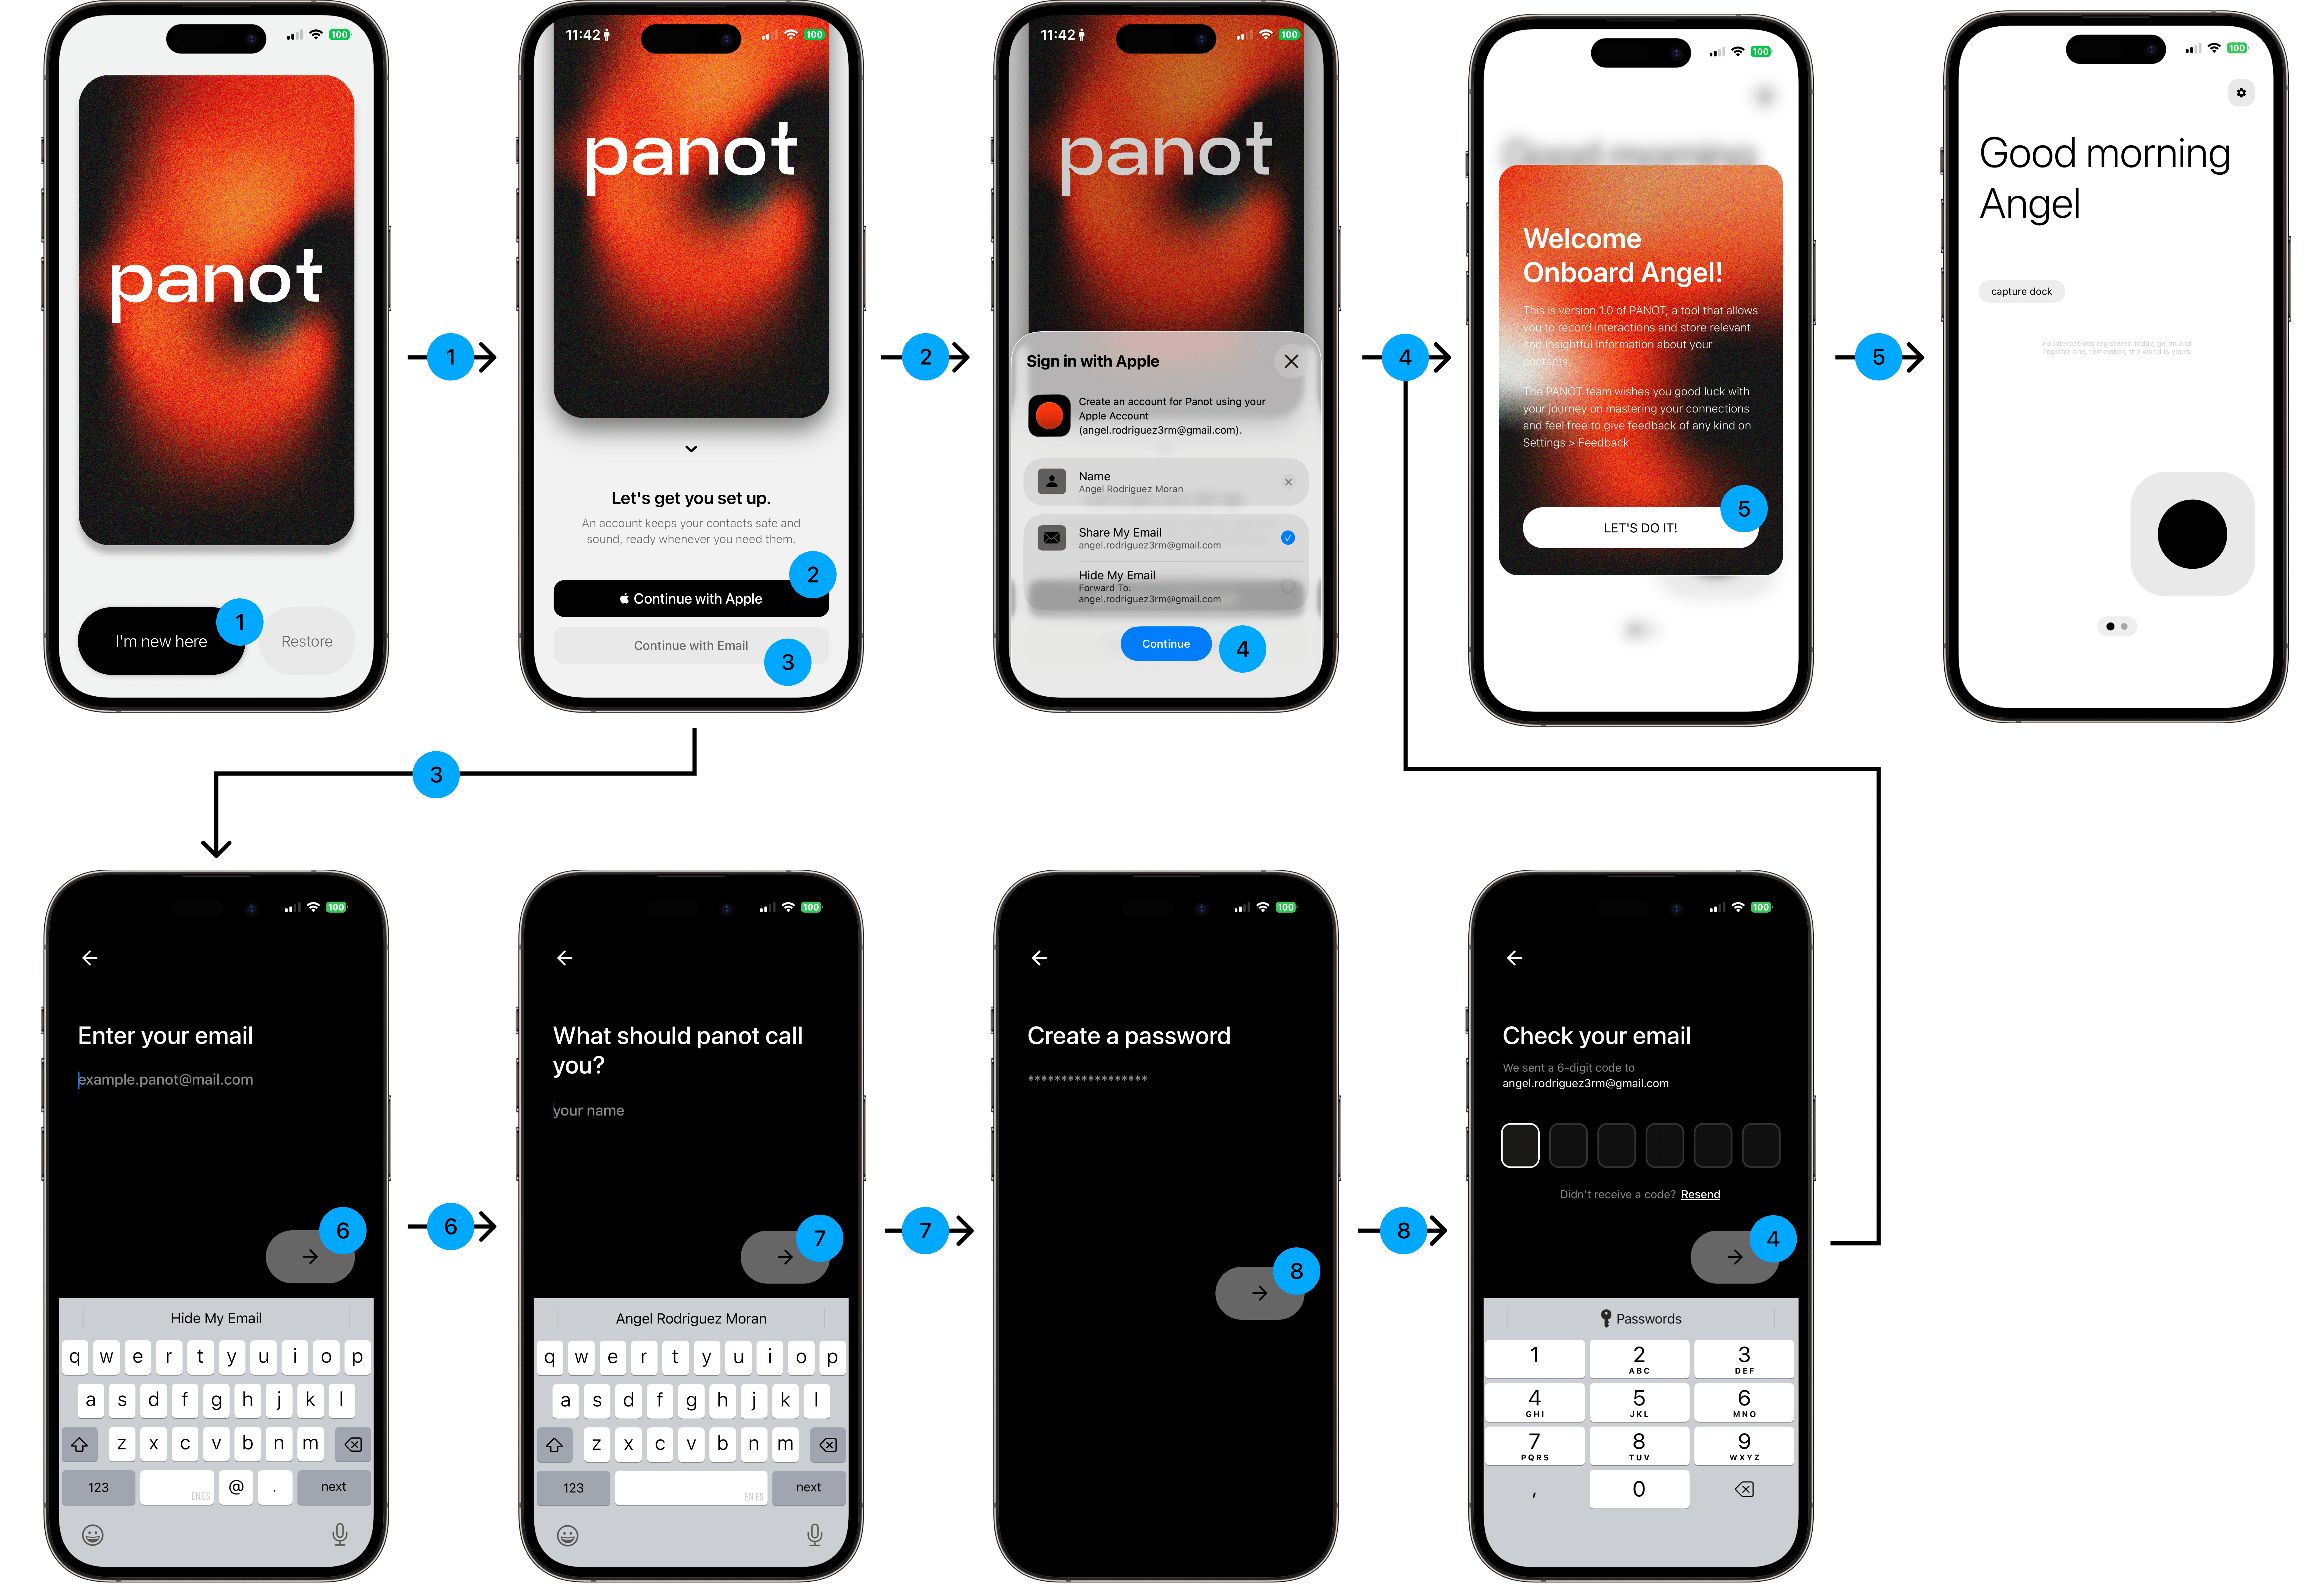
\includegraphics[width=0.8\textwidth]{figures/user-flow-onboarding.png}
    \caption{Flujo de Registro de Usuario y Onboarding}
    \label{fig:onboarding}
\end{figure}

\subsubsection{Flujo de Inicio de Sesión - \hyperref[req:HU-01]{HU-01}}

\begin{figure}[H]
    \centering
    \includegraphics[width=0.75\textwidth]{figures/user-flow-signin.png}
    \caption{Flujo de Inicio de Sesión}
    \label{fig:signin}
\end{figure}

Ambos flujos de Registro \ref{fig:onboarding} e Inicio de Sesión \ref{fig:signin} recogen la posibilidad de que el usuario use su \textit{Correo electrónico} o su \textit{Apple ID} como proveedor de autenticación.

\vspace{3.5cm}
\subsubsection{Flujo de Creación de Contacto - \hyperref[req:HU-02]{HU-02} y \hyperref[req:HU-03]{HU-03}}

El siguiente flujo de ususario abarca las tres posibilidades de creación de un contacto: creación manual (camino \textit{1 - 2 - 4 - 9}), creación con dictado (camino \textit{1 - 2 - 5 - 10 - 11}) e 
importación del contacto (camino \textit{1 - 2 - 6 - 7-  8}).

\begin{figure}[H]
    \centering
    \includegraphics[width=0.8\textwidth]{figures/user-flow-new-contact.png}
    \caption{Flujo de Creación de Contacto}
    \label{fig:new-contact}
\end{figure}

Para validar el funcionamiento de este proceso, se ha analizado la orquestación interna del sistema tras la creación del contacto \textbf{Pedro}. Como se observa en la Figura \ref{fig:trace-pedro}, 
el motor multi-agente inicia una traza de ejecución para crear el nuevo contacto con su grafo contextual correspondiente.

\begin{figure}[H]
    \centering
    \includegraphics[width=0.9\textwidth]{figures/traza-ejemplo-pedro.png}
    \caption{Traza de ejecución en LangSmith para la creación del contacto \textbf{Pedro}.}
    \label{fig:trace-pedro}
\end{figure}

El resultado es el siguiente grafo semántico (ver Figura \ref{fig:grafo-pedro}) donde el contacto no es una entrada tabular, sino el nodo central de una red de conceptos.

\begin{figure}[H]
    \centering
    \includegraphics[width=0.5\textwidth]{figures/grafo-inicial-pedro.png}
    \caption{Grafo de conocimiento resultante de la creación del contacto \textbf{Pedro}.}
    \label{fig:grafo-pedro}
\end{figure}


Posteriormente, al crear el contacto \textbf{Pepe}, el sistema activa el \textit{matching semántico} para identificar nodos comunese entre los contactos. Como se evidencia en la Figura \ref{fig:grafo-pedro-pepe-inicial}, el sistema 
ha identificado de forma autónoma que ambos tienen los nodos comunes \textbf{Universidad Complutense} y \textbf{pádel}, estableciendo una conexión relacional entre los dos contactos sin intervención del usuario.

\begin{figure}[H]
    \centering
    \includegraphics[width=0.8\textwidth]{figures/grafo-pedro-pepe.png}
    \caption{Grafo de conocimiento resultante de la creación del contacto \textbf{Pepe} y la detección de nodos comunes con el contacto \textbf{Pedro}.}
    \label{fig:grafo-pedro-pepe-inicial}
\end{figure}

\vspace{.5cm}
\subsubsection{Flujo de Grabación y Procesamiento de Interacción - \hyperref[req:HU-04]{HU-04}, \hyperref[req:HU-06]{HU-06} y \hyperref[req:HU-08]{HU-08}}

Los siguientes flujos de creación y procesamiento de una interacción que se exponene a continuación corresponden dos variantes: la primera (\hyperref[fig:new-interaction-long]{I}) corresponde a asignación de la interacción a un 
contacto previo a aceptar la creación de la interacción. Mientras que la segunda (\hyperref[fig:new-interaction-short]{II}) corresponde a la creación de una nueva interacción sin asignarla a un contacto previamente.

\begin{figure}[H]
    \centering
    \includegraphics[width=0.8\textwidth]{figures/user-flow-new-interaction-long.png}
    \caption{Flujo de Grabación y Procesamiento de Interacción (I)}
    \label{fig:new-interaction-long}
\end{figure}

\begin{figure}[H]
    \centering
    \includegraphics[width=0.8\textwidth]{figures/user-flow-new-interaction-short.png}
    \caption{Flujo de Grabación y Procesamiento de Interacción (II)}
    \label{fig:new-interaction-short}
\end{figure}

La Figura \ref{fig:grafo-pedro-pepe-nueva-interaccion} muestra el grafo tras procesar las interacciones reflejando la actualización e incorporación 
de los nuevos nodos concepto en ambos contactos.

\vspace{.5cm}
\begin{figure}[H]
    \centering
    \includegraphics[width=0.9\textwidth]{figures/grafo-pedro-pepe-ni.png}
    \caption{Grafo de conocimiento resultante de los contactos \textbf{Pepe} y \textbf{Pedro} tras procesar las nuevas interacciones.}
    \label{fig:grafo-pedro-pepe-nueva-interaccion}
\end{figure}

\newpage
\subsubsection{Flujo de Soporte y Feedback - \hyperref[req:HU-09]{HU-09}}

El siguiente flujo corresponde al envío de un ticket de soporte para un bug (camino \textit{1 - 2 - 4 - 6 - 7}) o una sugerencia (camino \textit{1 - 2 - 3 - 5 - 6 - 7}).

\begin{figure}[H]
    \centering
    \includegraphics[width=0.87\textwidth]{figures/user-flow-support.png}
    \caption{Flujo de Soporte y Feedback}
    \label{fig:support-feedback}
\end{figure}

Para cerrar el ciclo de soporte, se ha verificado la recepción de estos tickets en la base de datos. La Figura \ref{fig:db-tickets} muestra los registros reales en la tabla {\footnotesize \texttt{feedback\_tickets}} de Supabase, 
confirmando que el reporte de errores y sugerencias llega correctamente al equipo de desarrollo para su gestión.

\vspace{.5cm}
\begin{figure}[H]
    \centering
    \includegraphics[width=1\textwidth]{figures/db-feedback-tickets.png}
    \caption{Verificación de persistencia: Filas de la base de datos con los tickets de soporte enviados.}
    \label{fig:db-tickets}
\end{figure}

\subsubsection{Flujo de Configuración y Ajustes}

\begin{figure}[H]
    \centering
    \includegraphics[width=0.8\textwidth]{figures/user-flow-settings.png}
    \caption{Flujo de Configuración y Ajustes}
    \label{fig:configuracion-ajustes}
\end{figure}
\section{Verificación de Requisitos}

Una vez expuestos los resultados visuales y técnicos del sistema, se procede a la verificación formal de los requisitos definidos en la fase de análisis. Este proceso asegura que el artefacto 
desarrollado cumple con la especificación original y garantiza los niveles de calidad exigidos.

\subsection{Verificación de Requisitos Funcionales}

Para validar la funcionalidad del sistema, se ha realizado un contraste entre cada requisito funcional y la evidencia generada en los flujos de usuario. En la siguiente tabla se detalla 
el estado de cumplimiento de cada requisito, vinculándolos con los flujos de la sección anterior.

\begin{table}[H]
\centering
\scriptsize
\begin{tabularx}{\textwidth}{|l|X|c|l|}
\hline
\rowcolor[HTML]{EFEFEF} 
\textit{ID} & \textit{Descripción del Requisito} & \textit{Estado} & \textit{Evidencia / Fuente} \\ \hline
\textbf{\hyperref[req:FR-01]{FR-01}} & Registro e inicio de sesión seguro. & Logrado & Flujos \ref{fig:onboarding} y \ref{fig:signin} \\ \hline
\textbf{\hyperref[req:FR-02]{FR-02}} & Cerrar sesión del usuario de forma segura. & Logrado & Flujo \ref{fig:configuracion-ajustes} \\ \hline
\textbf{\hyperref[req:FR-03]{FR-03}} & Eliminación completa de cuenta y datos. & Logrado &  Flujo \ref{fig:configuracion-ajustes} \\ \hline
\textbf{\hyperref[req:FR-04]{FR-04}} & Creación de un contacto manualmente. & Logrado & Flujo \ref{fig:new-contact} \\ \hline
\textbf{\hyperref[req:FR-05]{FR-05}} & Importación de contactos desde agenda nativa. & Logrado & Flujo \ref{fig:new-contact} \\ \hline
\textbf{\hyperref[req:FR-06]{FR-06}} & Creación de contacto mediante dictado de voz. & Logrado & Flujo \ref{fig:new-contact}, Traza \ref{fig:trace-pedro} y Fig. \ref{fig:grafo-pedro} \\ \hline
\textbf{\hyperref[req:FR-07]{FR-07}} & Búsqueda semántica y por nombre. & Logrado & Barra de búsqueda (Flujo \ref{fig:new-contact}) \\ \hline
\textbf{\hyperref[req:FR-10]{FR-10}} & Interfaz dedicada de grabación y aceptación de permisos de hardware. & Logrado & Flujos \ref{fig:new-interaction-long} y \ref{fig:new-interaction-short} \\ \hline
\textbf{\hyperref[req:FR-11]{FR-11}} & Validación de texto transcrito previo a aceptación. & Logrado & Flujos \ref{fig:new-interaction-long} y \ref{fig:new-interaction-short} \\ \hline
\textbf{\hyperref[req:FR-12]{FR-12}} & Conversión de audio a texto en tiempo real. & Logrado & Módulo {\scriptsize \texttt{panot-speech}} \\ \hline
\textbf{\hyperref[req:FR-13]{FR-13}} & Descartar una interacción. & Logrado & Flujos \ref{fig:new-interaction-long} y \ref{fig:new-interaction-short} \\ \hline
\textbf{\hyperref[req:FR-14]{FR-14}} & Actualización del grafo semántico tras interacción. & Logrado & Figuras \ref{fig:grafo-pedro-pepe-inicial} y \ref{fig:grafo-pedro-pepe-nueva-interaccion} \\ \hline
\textbf{\hyperref[req:FR-15]{FR-15}} & Generación de relaciones (matching semántico). & Logrado & Fig. \ref{fig:grafo-pedro-pepe-nueva-interaccion} (Nodos comunes) \\ \hline
\textbf{\hyperref[req:FR-16]{FR-16}} & Envío de reportes de errores o bugs. & Logrado & Flujo \ref{fig:support-feedback} y Fig.\ref{fig:db-tickets} \\ \hline
\textbf{\hyperref[req:FR-17]{FR-17}} & Envío de propuestas de mejora o solicitudes de nuevas funcionalidades. & Logrado & Flujo \ref{fig:support-feedback} y Fig. \ref{fig:db-tickets} \\ \hline
\end{tabularx}
\caption{Tabla de verificación del cumplimiento de Requisitos Funcionales. Se han omitido los requisitos \hyperref[req:FR-08]{FR-08} y \hyperref[req:FR-09]{FR-09} que corresponden a la edición y 
eliminación de un contacto por motivos de simplicidad de la memoria.}
\label{tab:verificacion-funcional}
\end{table}


\subsection{Verificación de Requisitos No Funcionales}

[VERIFICACIÓN DE REQUISITOS NO FUNCIONALES]
\section{Cumplimiento de Objetivos}

[CUMPLIMIENTO DE OBJETIVOS IMPUESTOS EN INTRO]
\chapter{Conclusiones y Trabajo Futuro}
\label{ch:conclusiones-y-trabajo-futuro}

%%%%%%%%%%%%%%%%%%%%%%%%%%%%%%%%%%%
% CONCLUSIONES GENERALES

\section{Conclusiones Generales}

[Escribir aquí las conclusiones generales]

%%%%%%%%%%%%%%%%%%%%%%%%%%%%%%%%%%%
% APLICACIÓN DE CONOCIMIENTOS ADQUIRIDOS EN EL GRADO

\section{Aplicación de Conocimientos Adquiridos en el Grado}

[Escribir aquí la aplicación de conocimientos adquiridos en el grado]

\input{chapter5-conclusiones/3-lineas-trabajo-futuro}


\end{document}
